\section{Simulation}\label{sec:Simulation}

% How can you verify the design and operation of your vehicle? For this, you can use the MATLAB/Simulink QSS toolbox and relevant vehicle equations.
% Overview of whole sim. process:
% --> To verify the design of the vehicle and all its subparts a model was built in QSS part for part during the design process
% First driving cycle + simple vehicle model (with parameters, that were already explained in the drive cycle design section, but simulation start and drive cycle design took part at same time)--> iterate and compare to analytical calculations --> add gearbox during designing of gbx and motors --> add EM, with custom Efficiency map (again some iterations and changes to the drivecycle were necessary) --> we get electrical power demand over time --> able to caculate energy demand between stops --> size and design battery --> model custom battery cells according to design with custom controller for LTO (see section energy source) --> complete charging model possible --> iterate and optimize AC charging lengths to stay in non critical SoC while least amount of AC charging necessary

%     What is the force-speed plot of the vehicle that can reflect its maximum speed, its operation at various gradients and its acceleration? Create your own, custom driving cycle in QSS toolbox that requests those values and verify the vehicle’s abilities. Include the plots in the report.
% --> force speed plot from analytical calculations with chosen vehicle parameters for max gradients and flat gradients
\begin{figure}[ht]
    \centering
    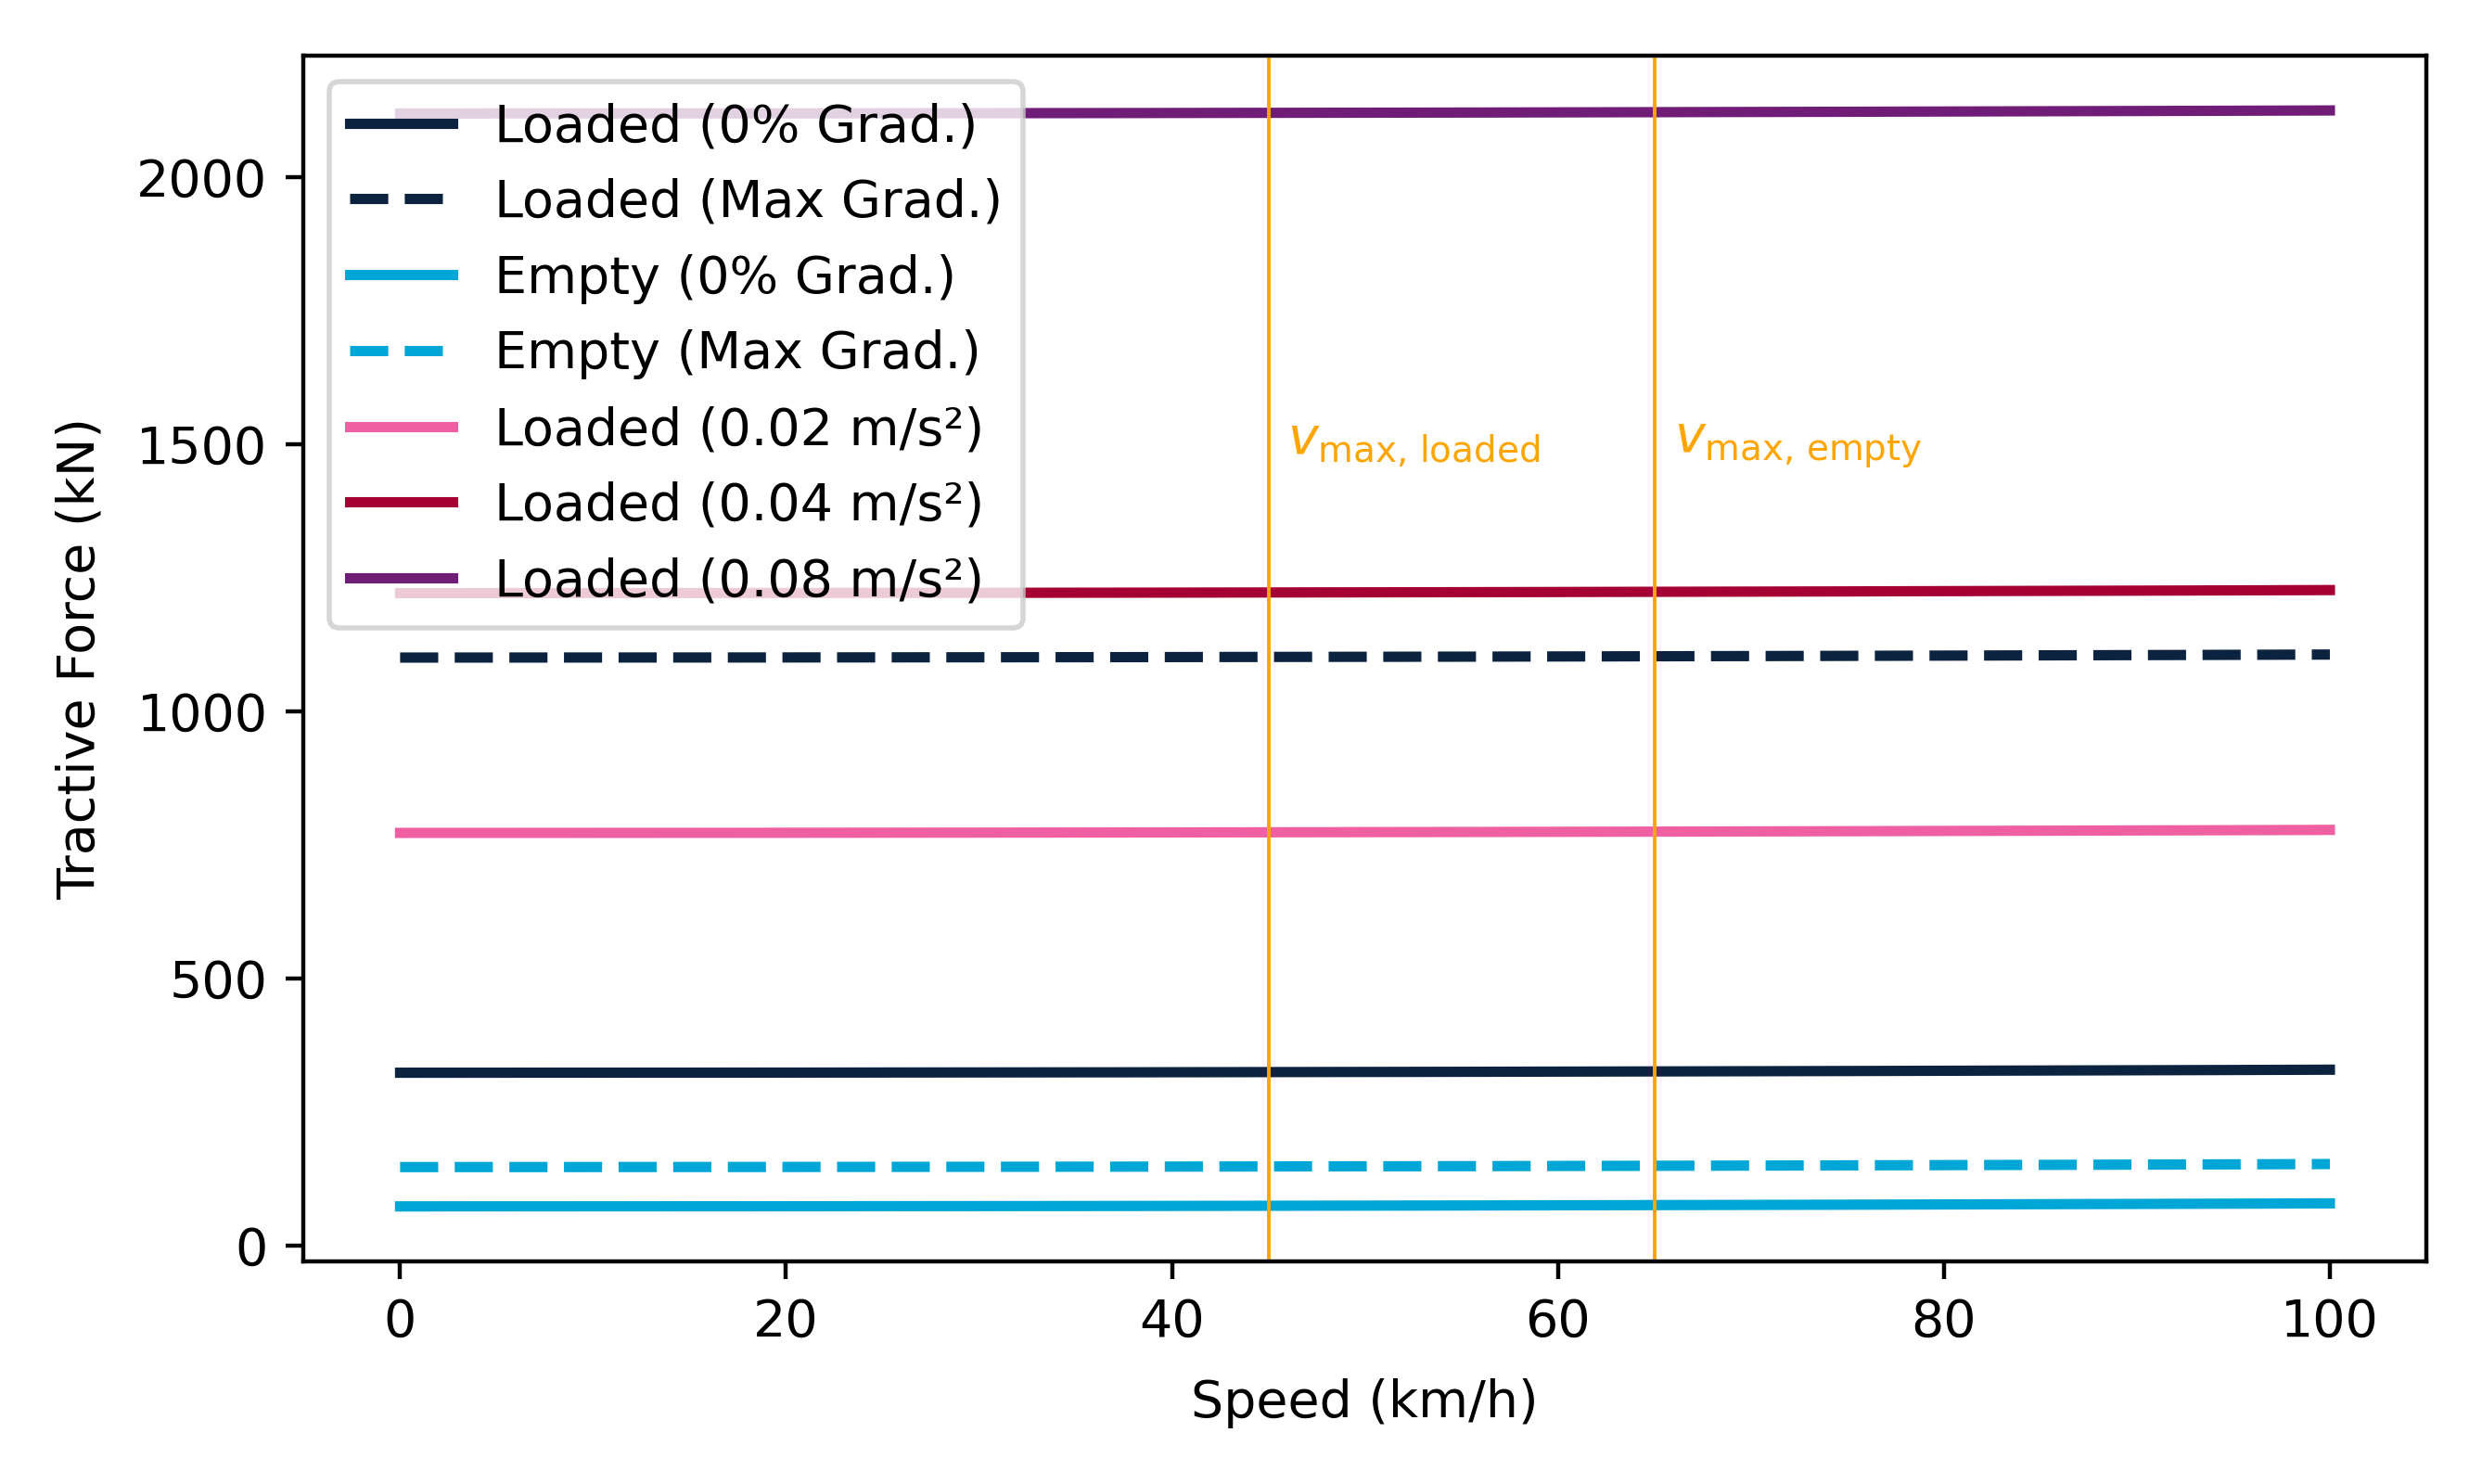
\includegraphics[]{EV_Project - Mauretanian Train/plots/tractive_force_vs_speed.png}
    \caption{Force-speed plot for the loaded and unloaded train with top speed at 0 and maximum gradient, as well as for the loaded train with the set acceleration levels at zero gradient.}
    \label{fig:force-speed}
\end{figure}
%     Is the vehicle able to achieve the designed acceleration, driving gradients, and top speed? If this is not the case, go back to your design steps (4-7) and see what needs to be changed.
% Since the entire driving cycle process was an iterative one that took place at the same time as designing the necessary output power for the engines, the designed vehicle specifications were met.
% The battery was designed more precisely later, after the finished motor design and its size was adjusted multiple times to match requirements. Since its an LTO battery it was not power, but purely energy limited in size (especially important for charging)
% Converters were also designed after the motor, when the electrical numbers were known

% Does the vehicle powertrain perform satisfactorily for the relevant drive cycles in terms of power and energy requirements? Make sure to use a representative driving cycle for your specific case study. In case you are using a bus as a vehicle you can use the “Braunschweig” driving cycle, or the “Orange County Transit Bus Cycle (US-OCTA)” for Orange County, California, US, available from the US National Renewable Energy Laboratory (NREL). In case you are using a specific utility vehicle, then you can always create your own, representative driving cycle. Make sure to use references and explain how you got the specific values used in the driving cycle.

% Show final important plots, such as total electric power curve, Eff maps with OPs, energy usages between stops and SoC of battery 
%--> Since all parts of the vehicle model are able to follow the simulation with the designed specific drive cycles,  the powertrain does indeed perform satisfactory and the goal of the design is reached: Delivering the iron ore in under 20h from the mines to the sea! (and 15h back)
\begin{figure}[ht]
    \centering
    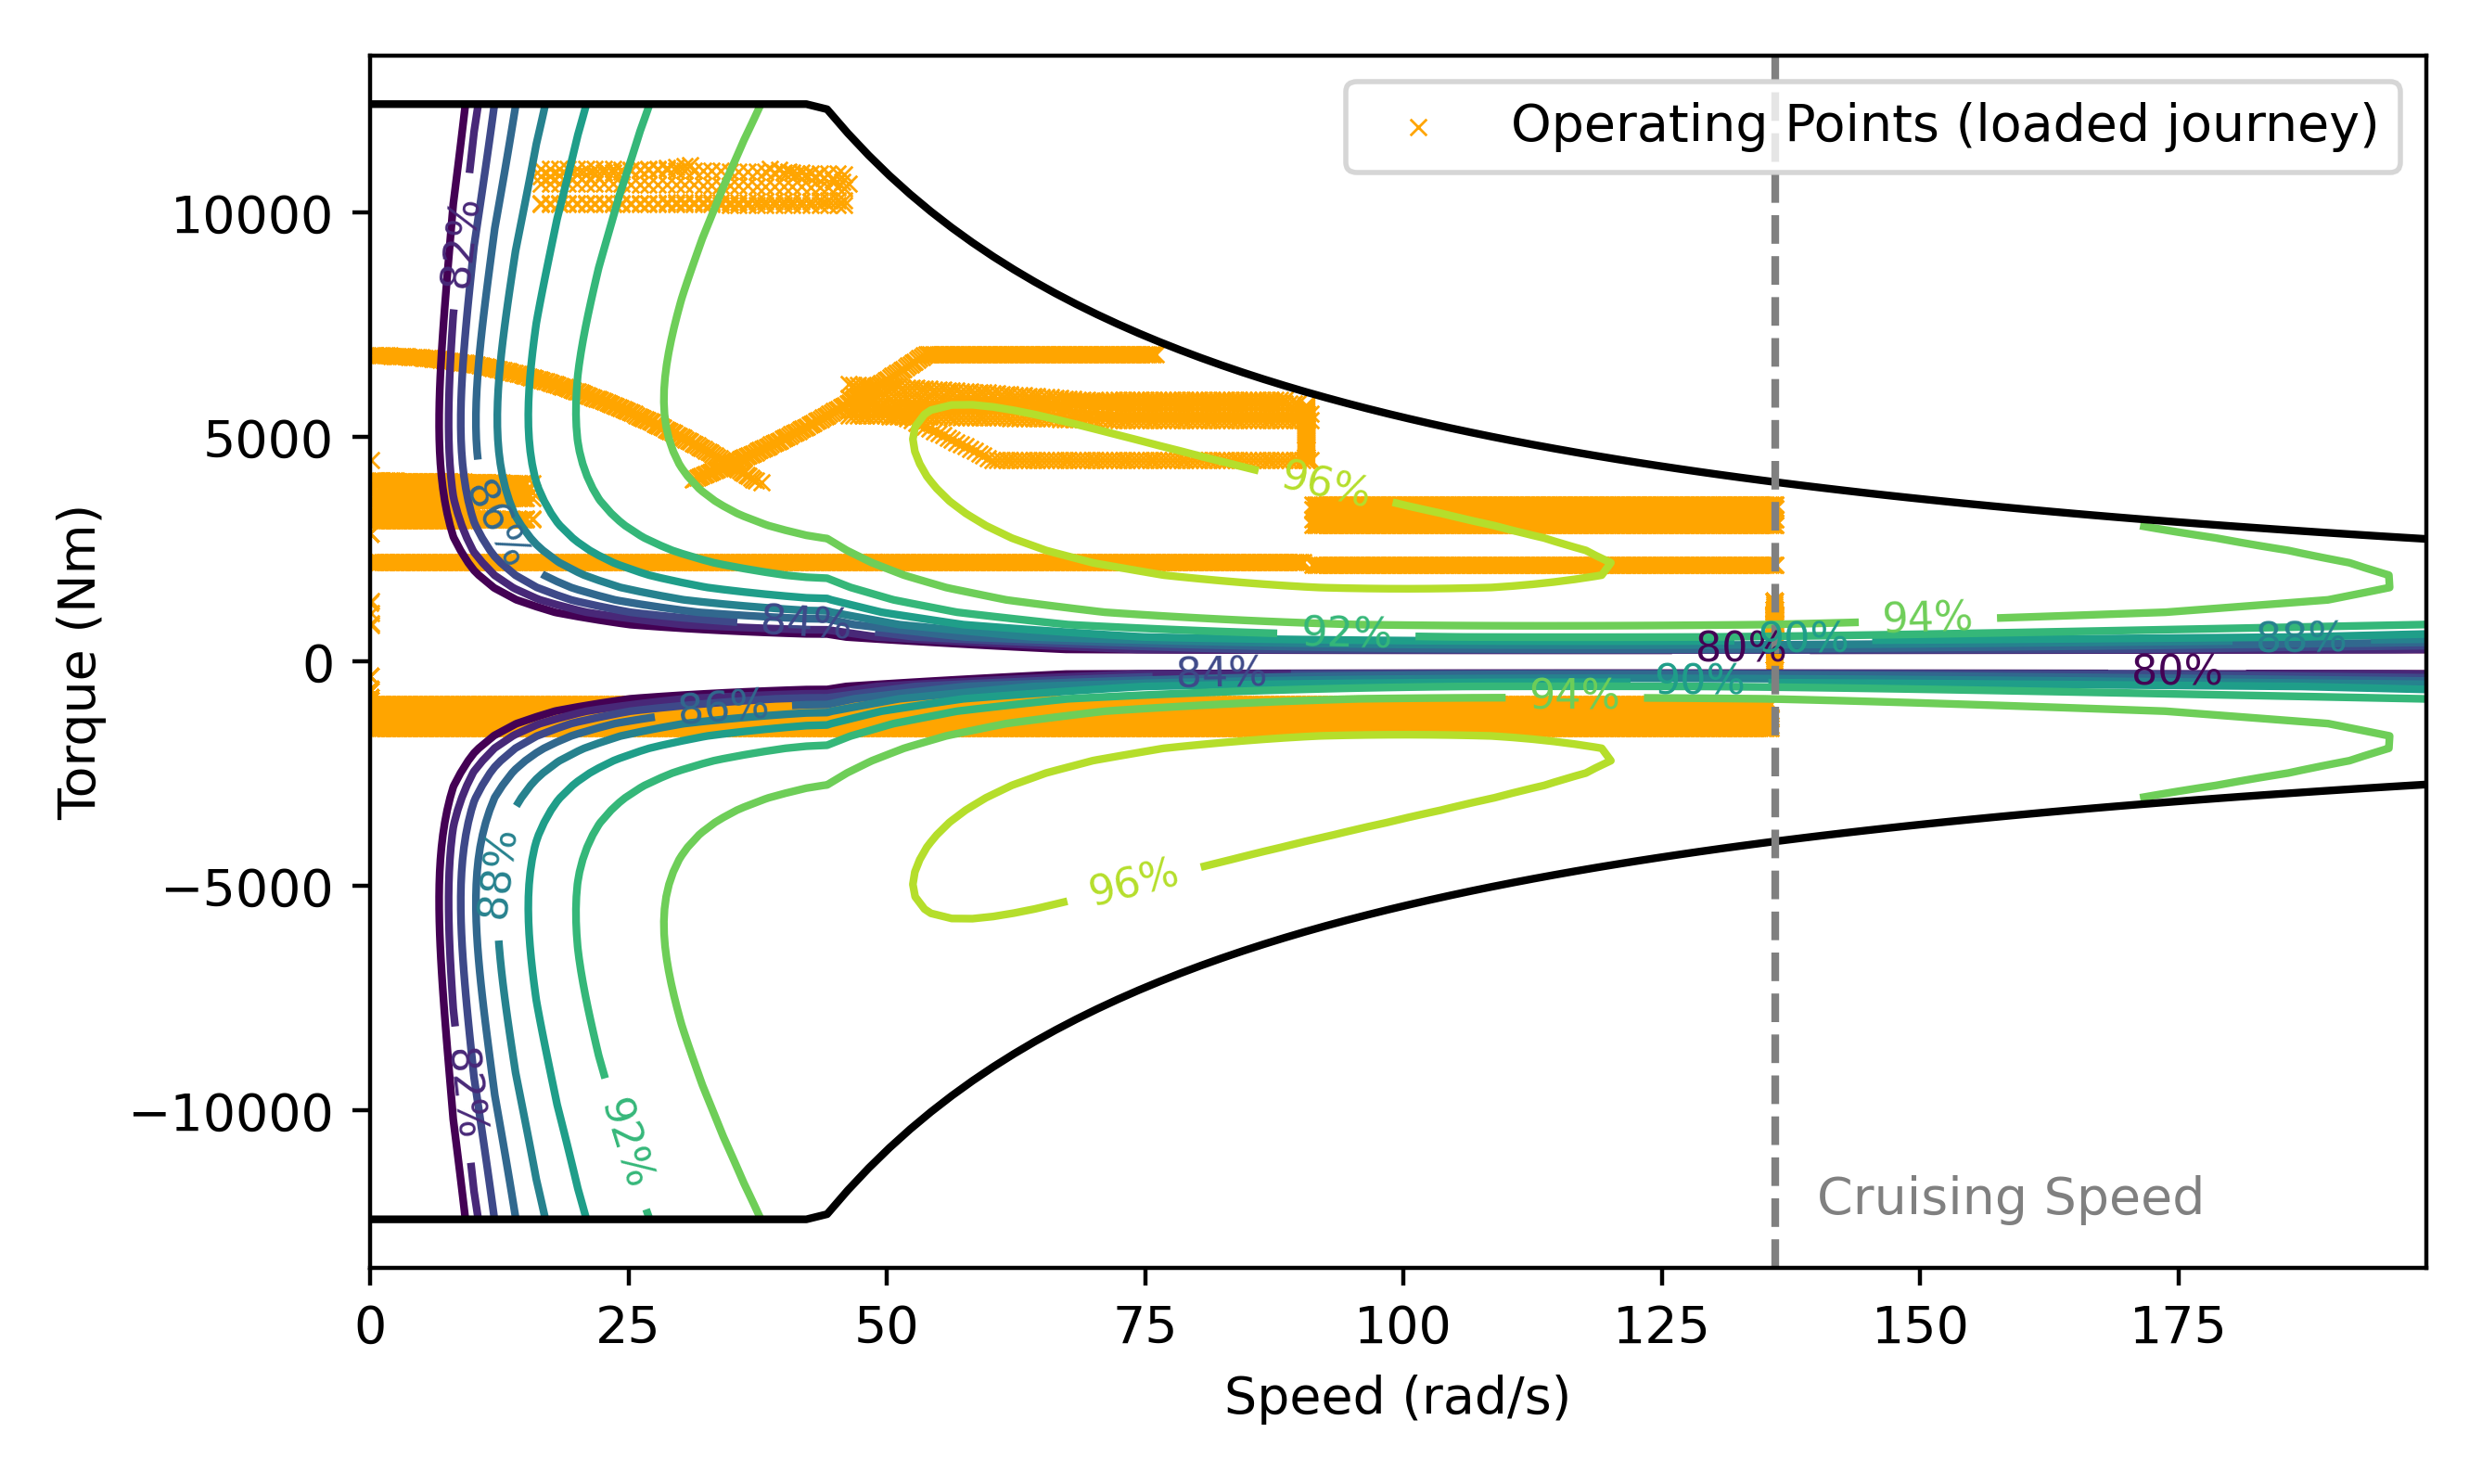
\includegraphics[]{EV_Project - Mauretanian Train/plots/efficiency_map_with_OPs_loaded.png}
    \caption{Efficiency map of the induction machine motors used in the train with the operating points for the loaded journey}
    \label{fig:eff_map_OPs_loaded}
\end{figure}

\begin{figure}[ht]
    \centering
    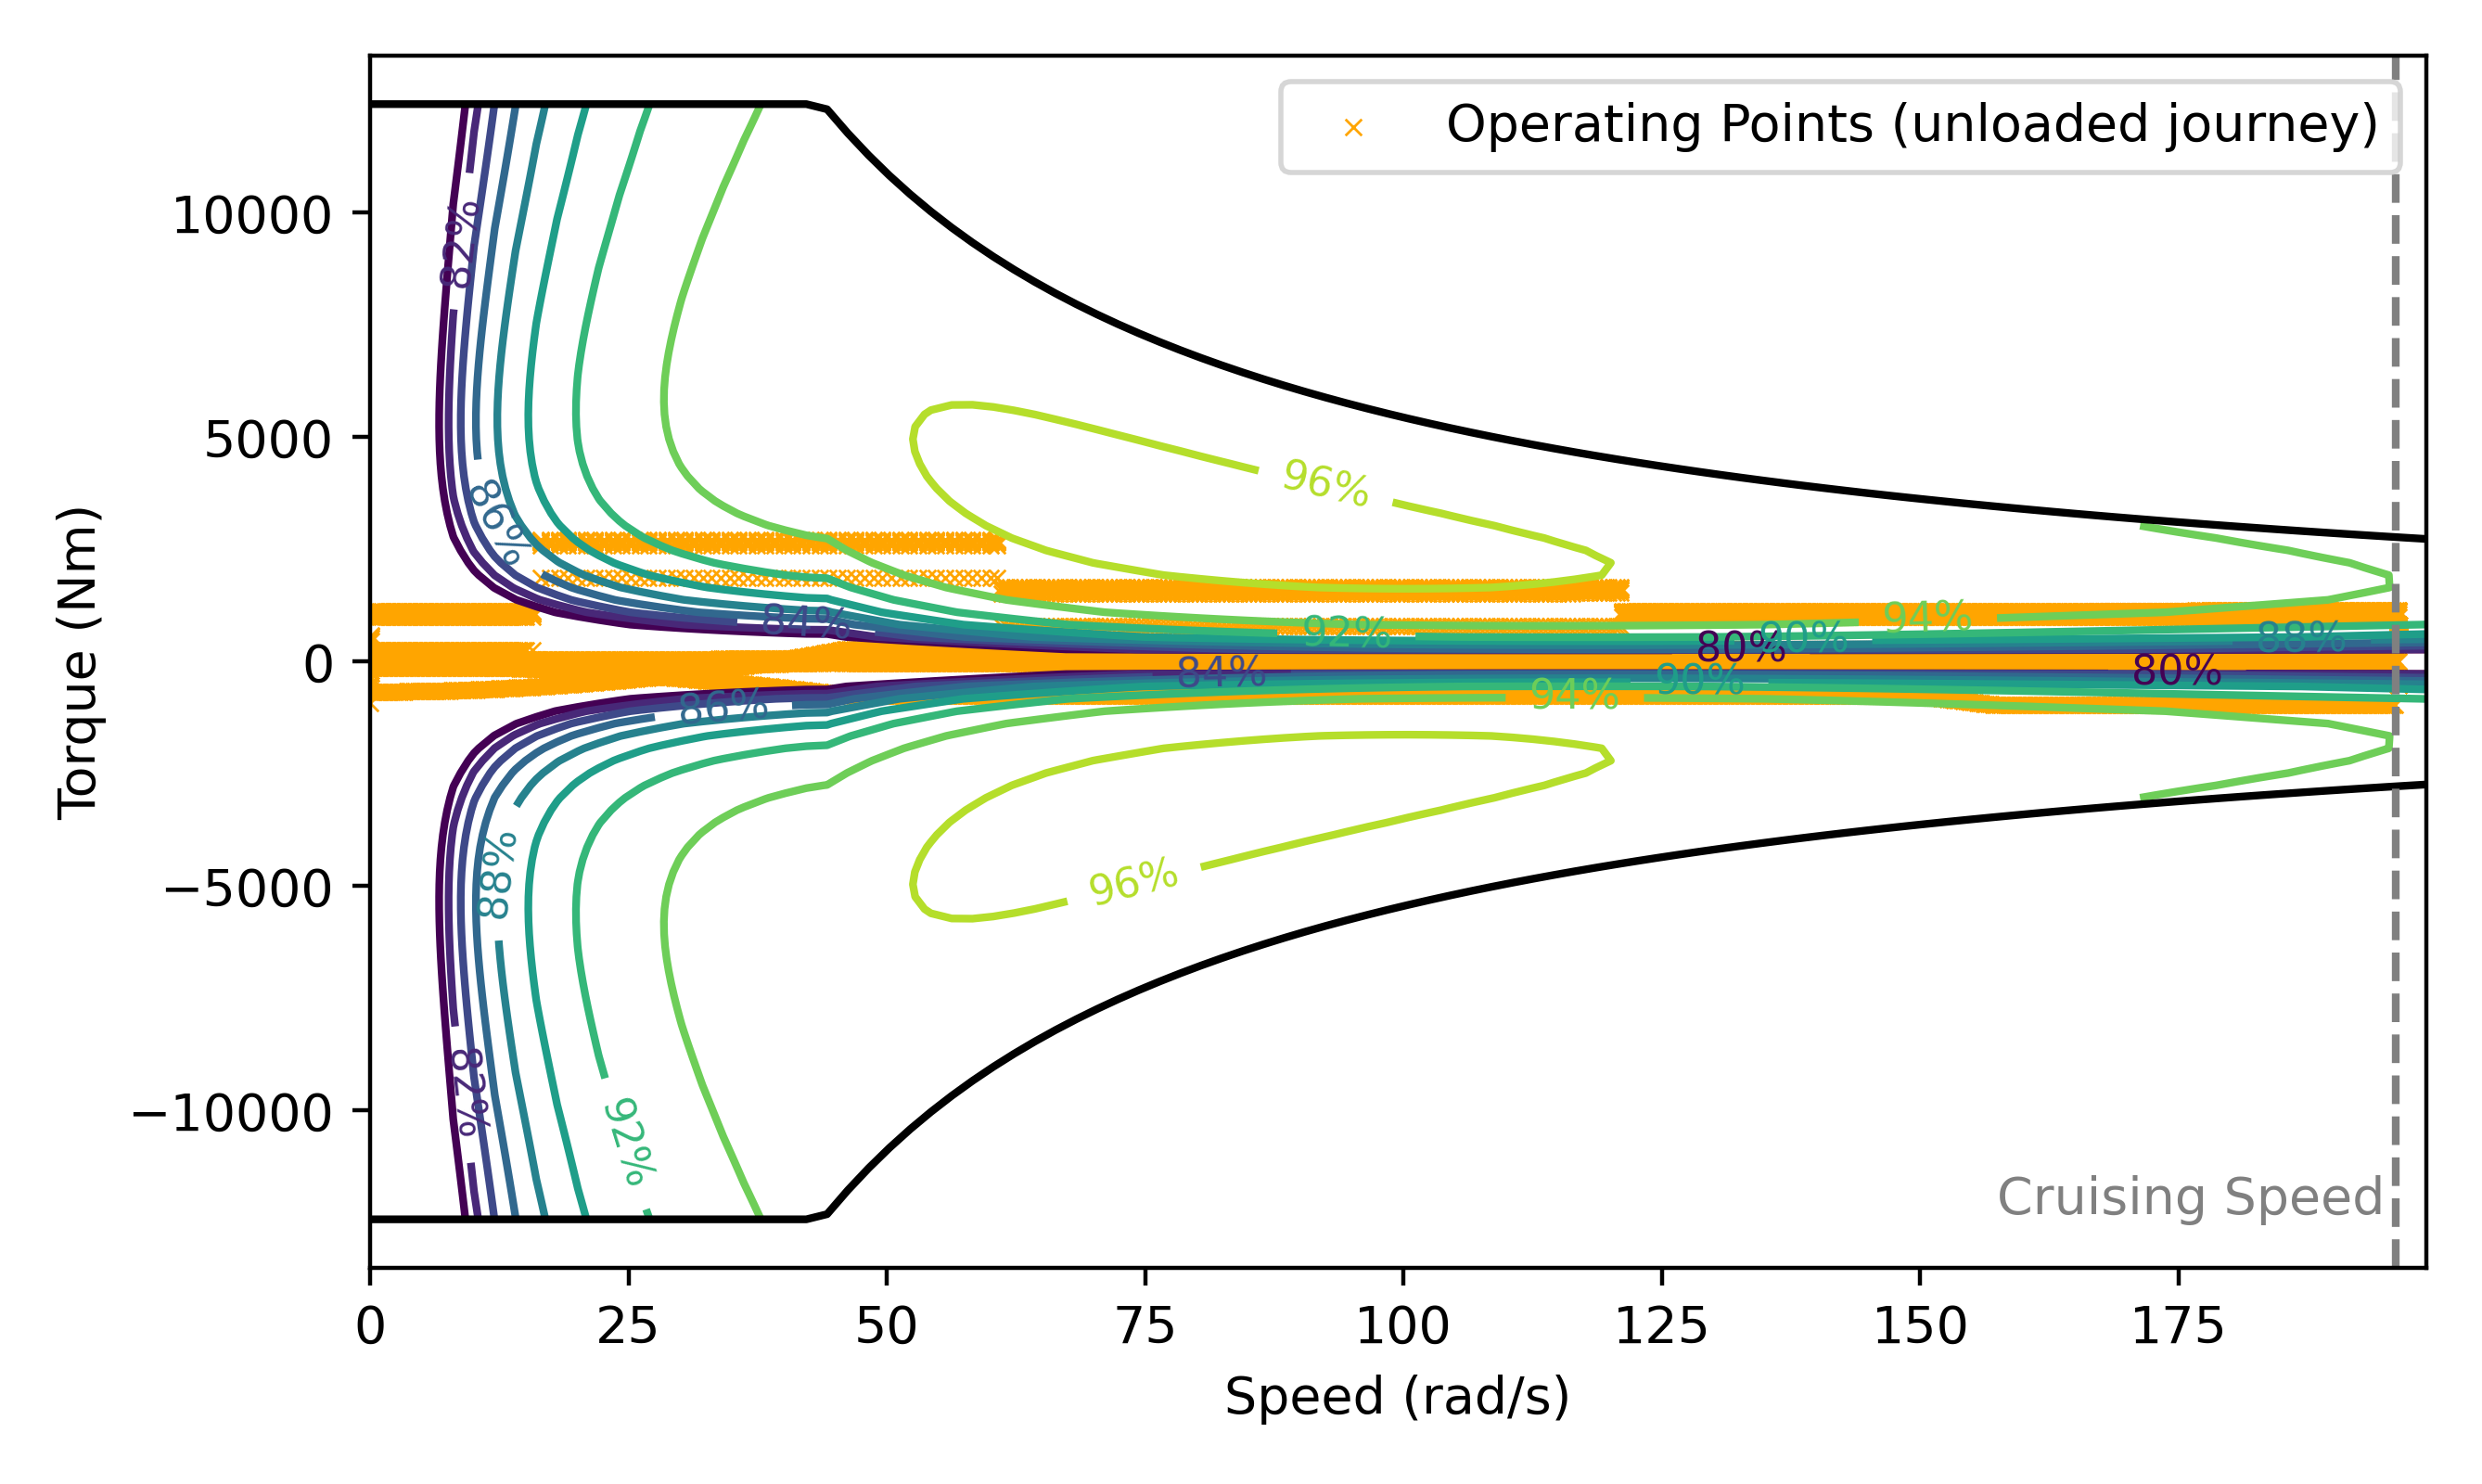
\includegraphics[]{EV_Project - Mauretanian Train/plots/efficiency_map_with_OPs_unloaded.png}
    \caption{Efficiency map of the induction machine motors used in the train with the operating points for the unloaded journey}
    \label{fig:eff_map_OPs_unloaded}
\end{figure}

\begin{figure}[ht]
    \centering
    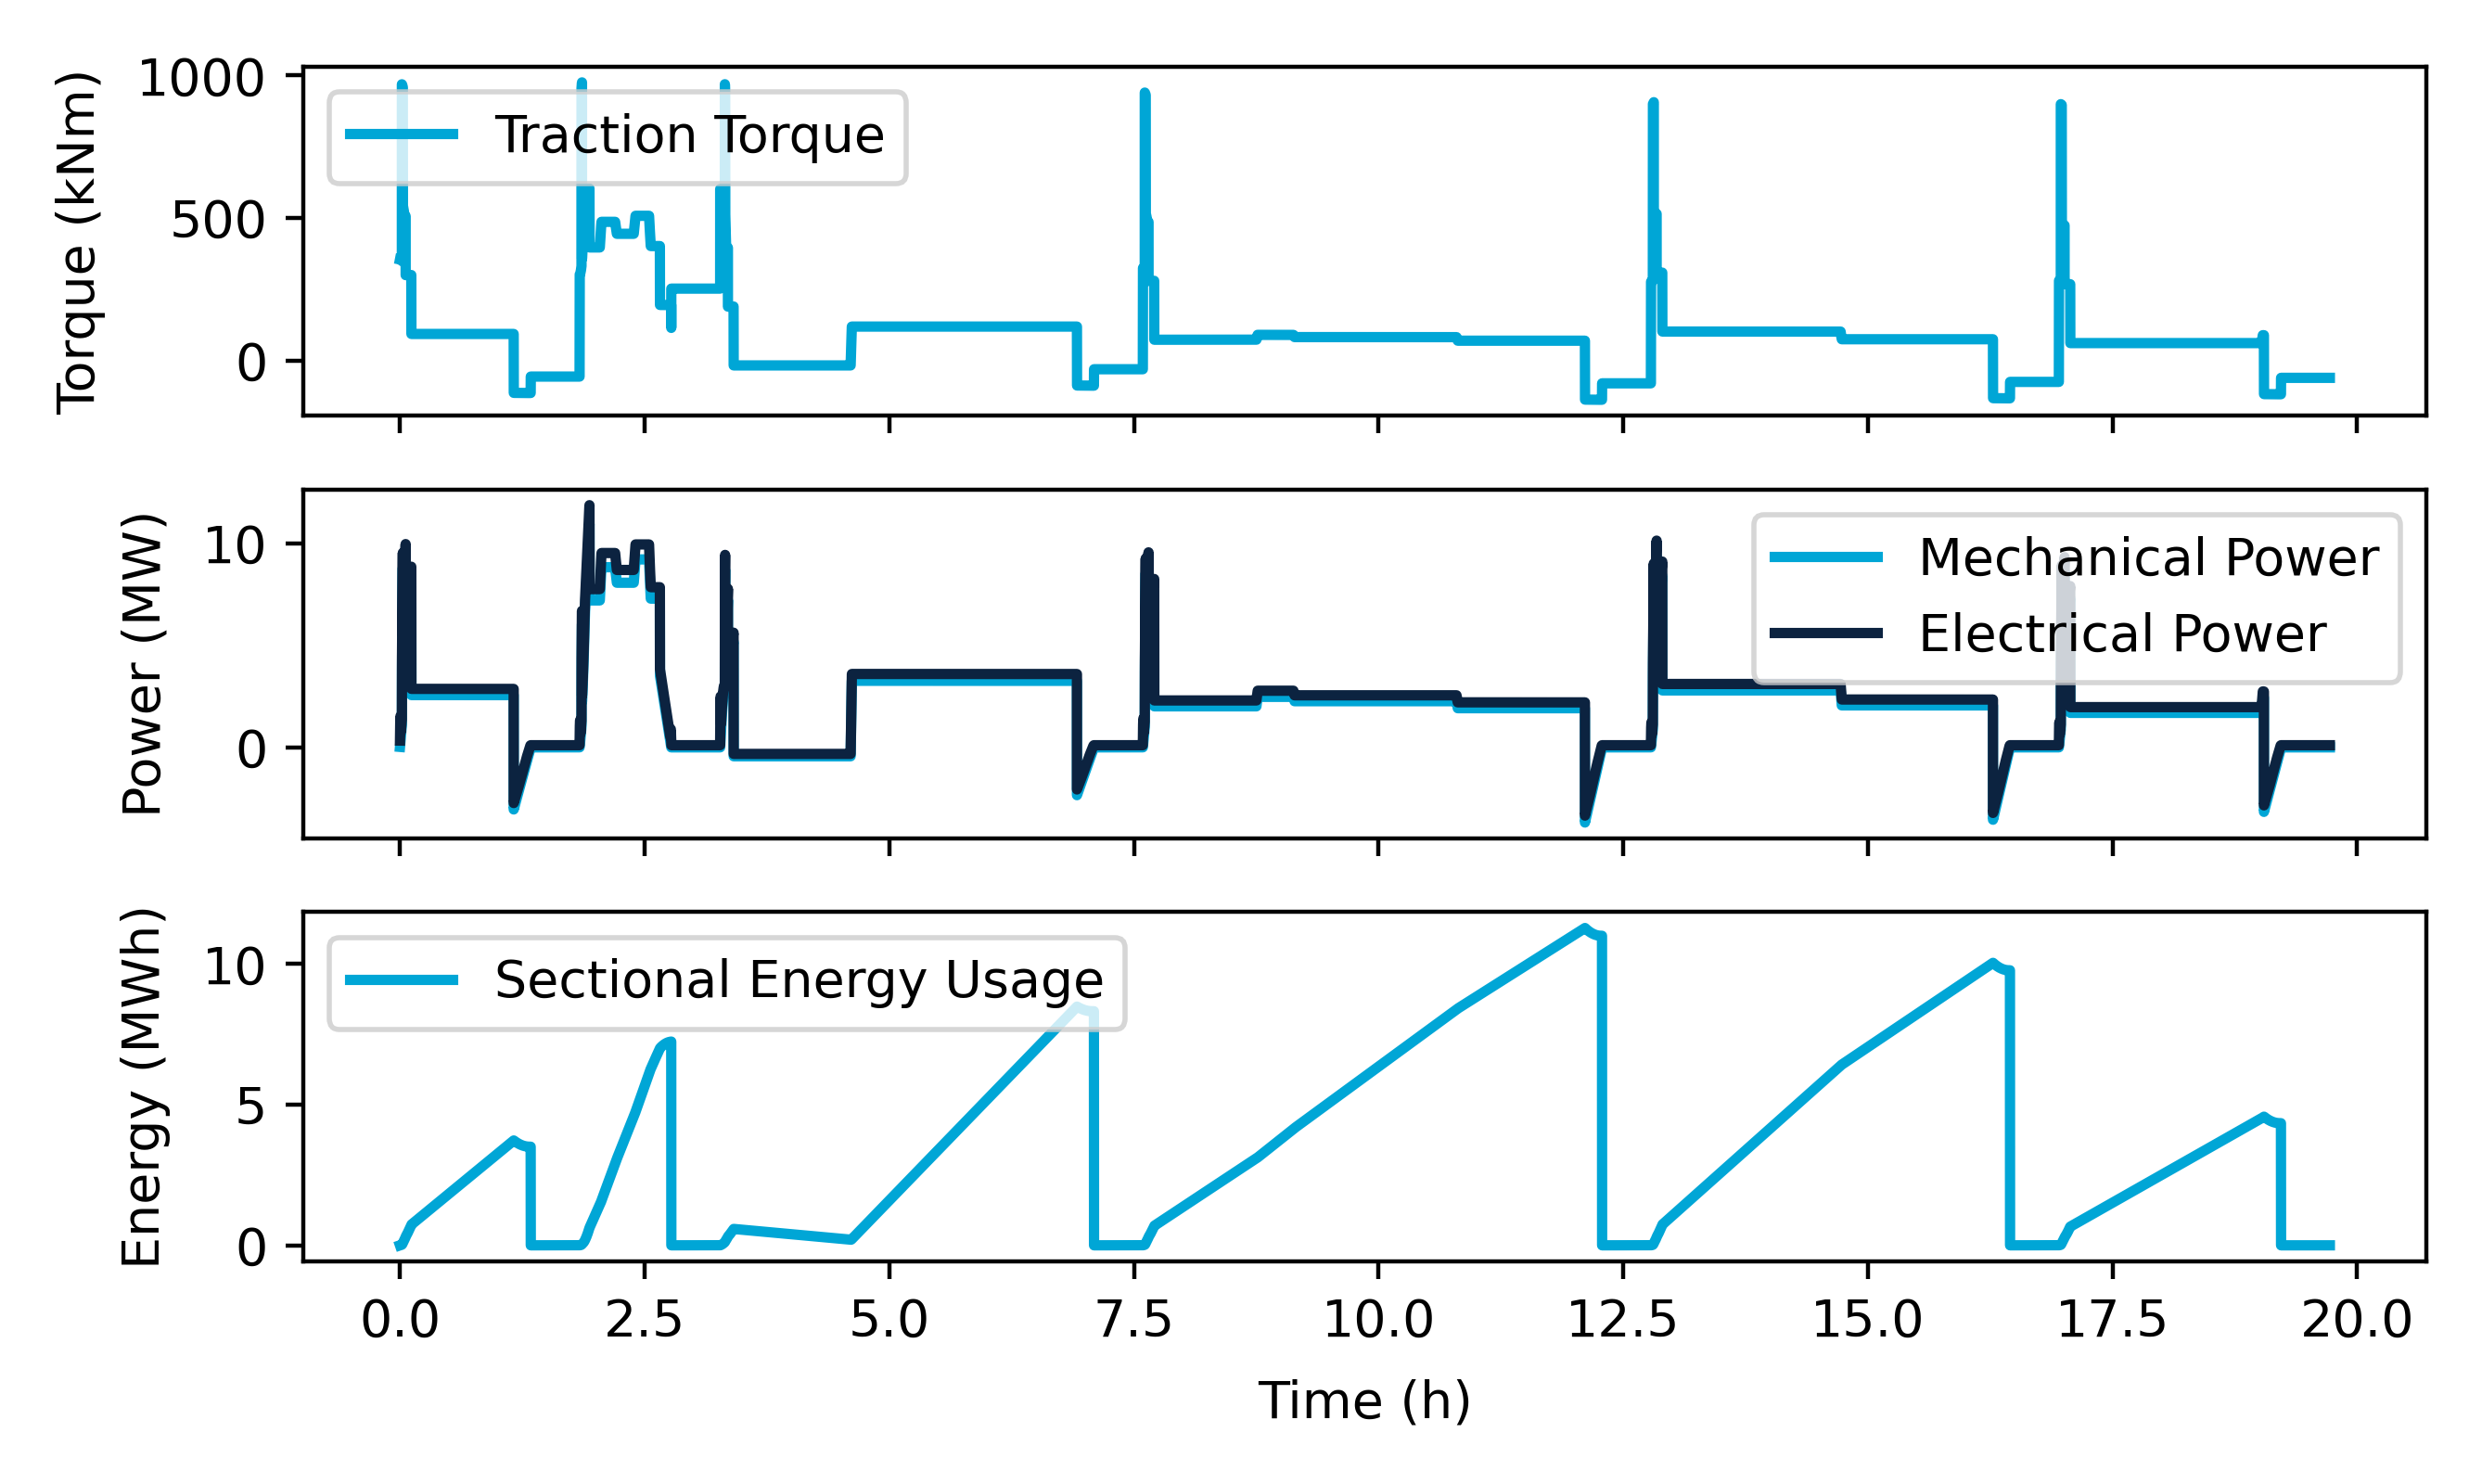
\includegraphics[]{EV_Project - Mauretanian Train/plots/power_energy_plots.png}
    \caption{Total tractive torque, the machines have to provide during the loaded journey, as well as tractive and electrical power that have to be provided and the resulting electrical energy that has to be provided by the battery in between the charging stops.}
    \label{fig:power_energy_loaded}
\end{figure}

\begin{figure}[ht]
    \centering
    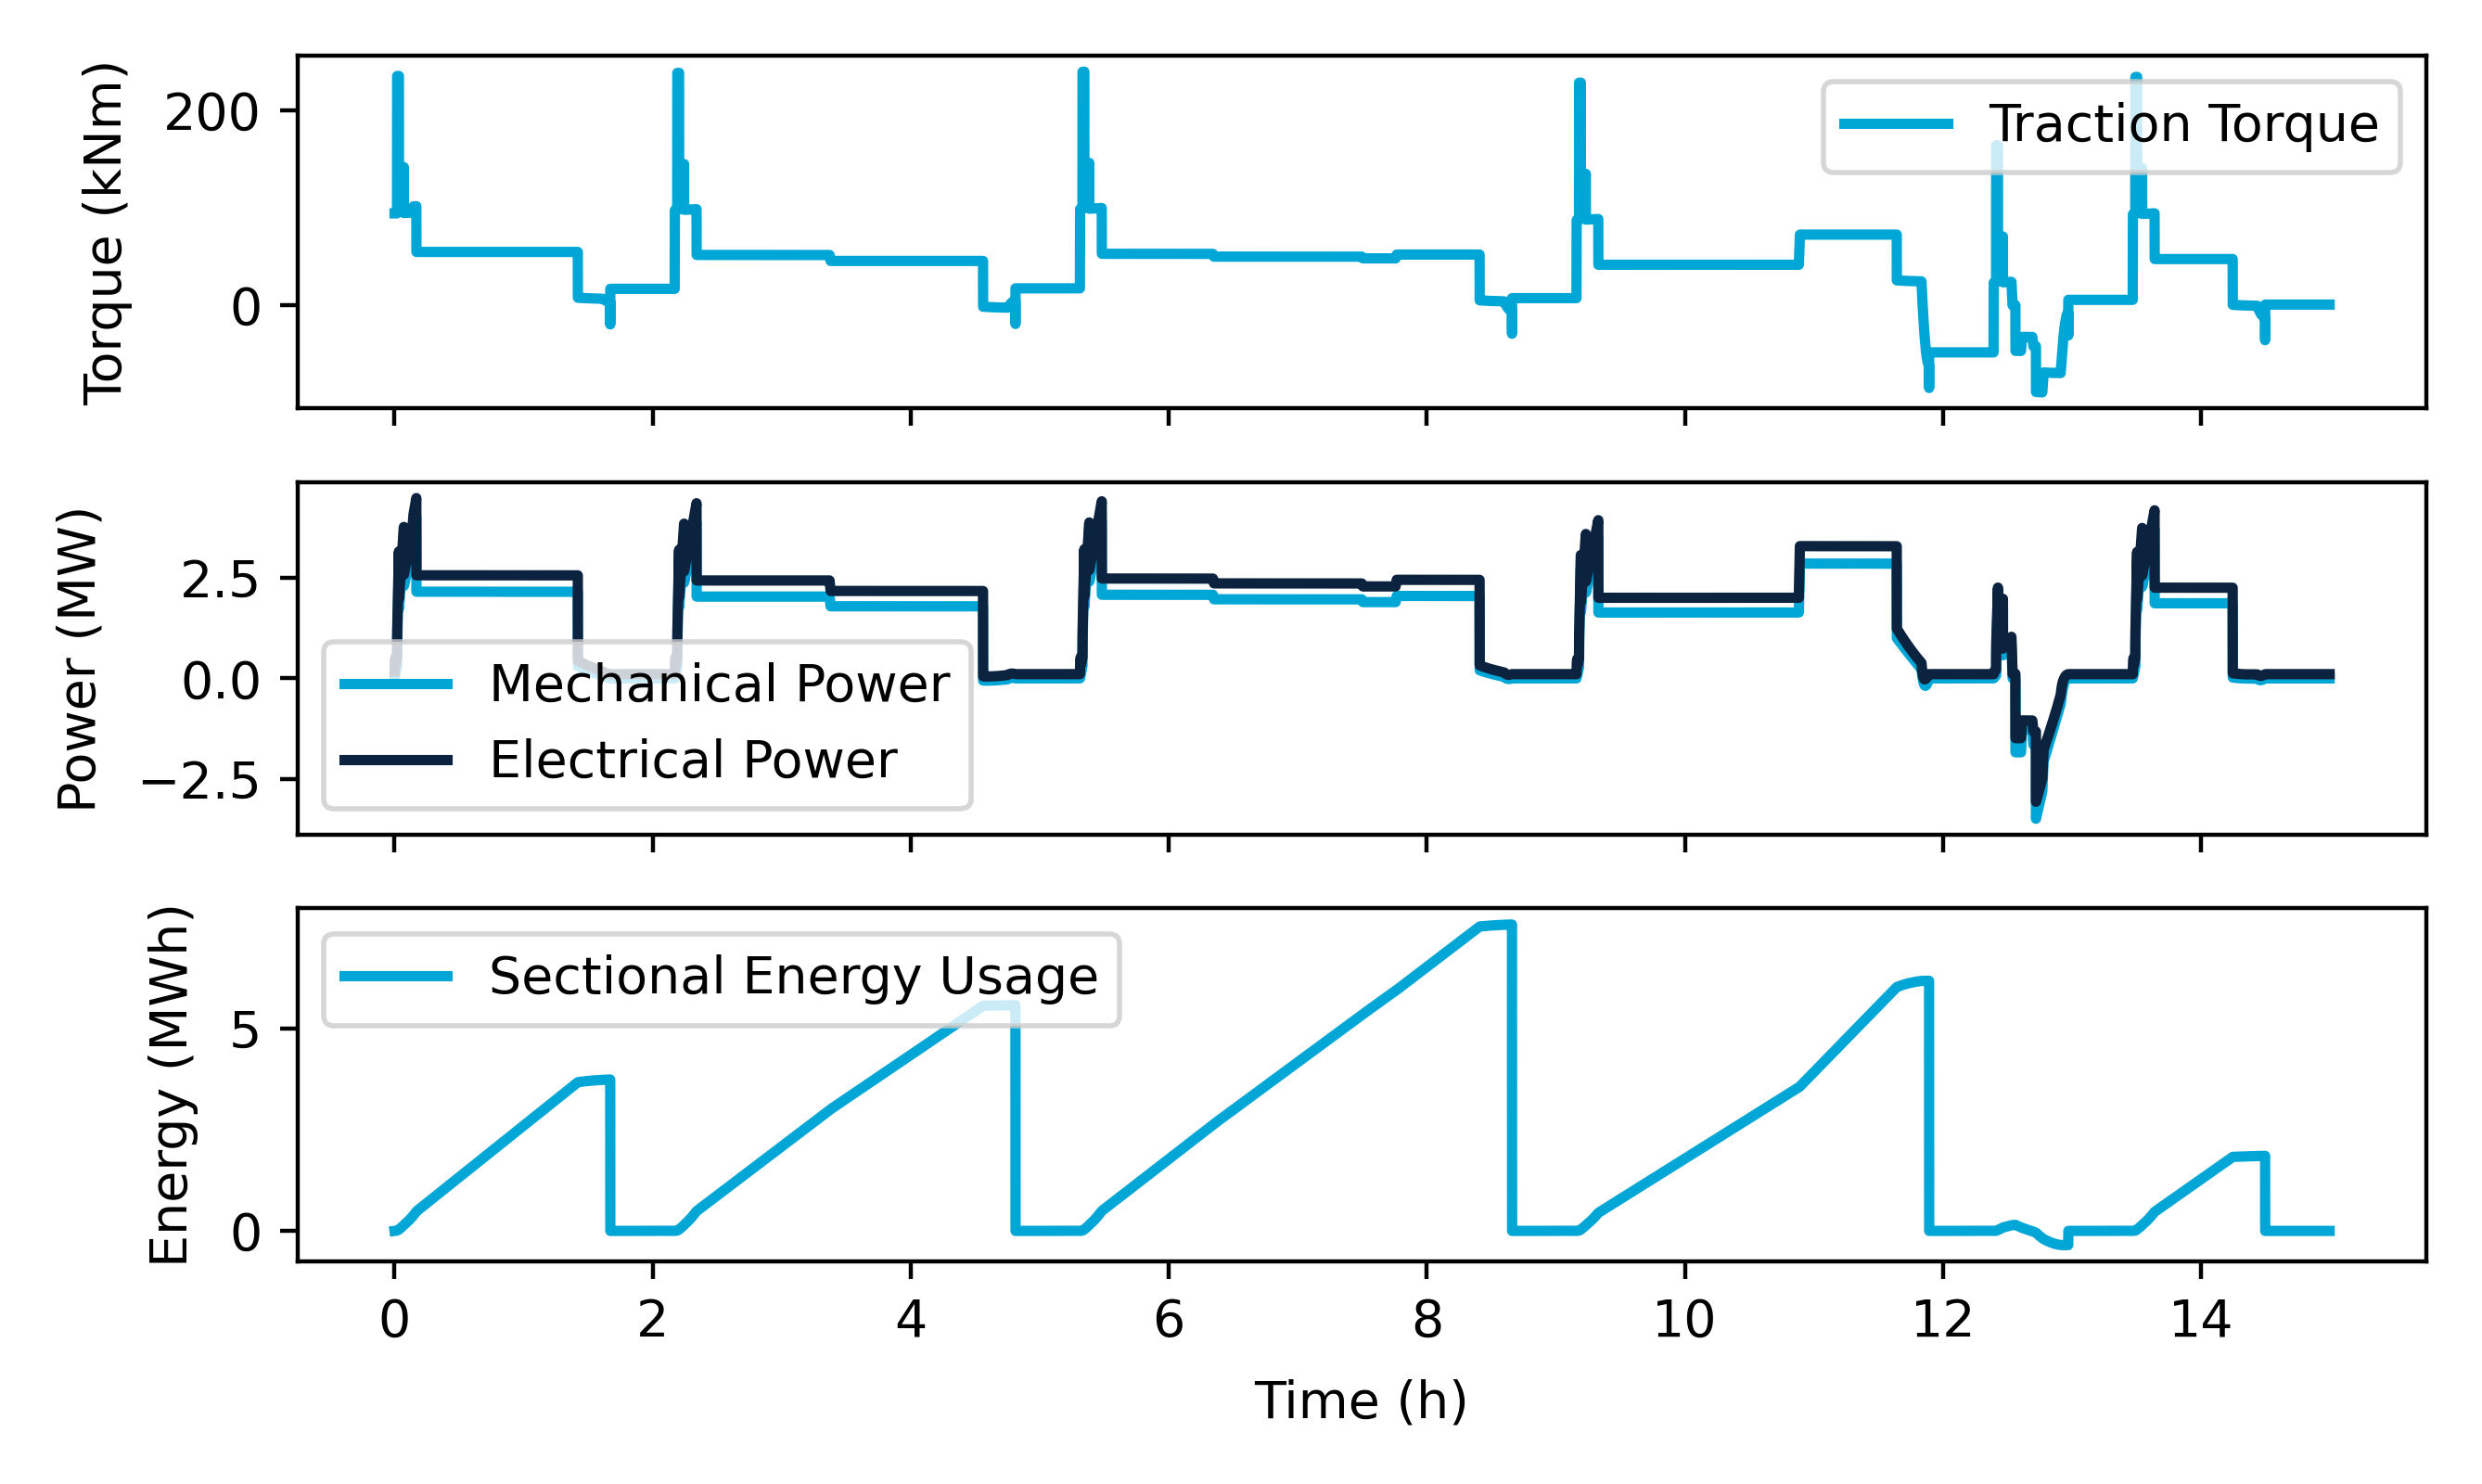
\includegraphics[]{EV_Project - Mauretanian Train/plots/power_energy_plots_unloaded.png}
    \caption{Total tractive torque, the machines have to provide during the loaded journey, as well as tractive and electrical power that have to be provided and the resulting electrical energy that has to be provided by the battery in between the charging stops.}
    \label{fig:power_energy_loaded}
\end{figure}

\begin{figure}[ht]
    \centering
    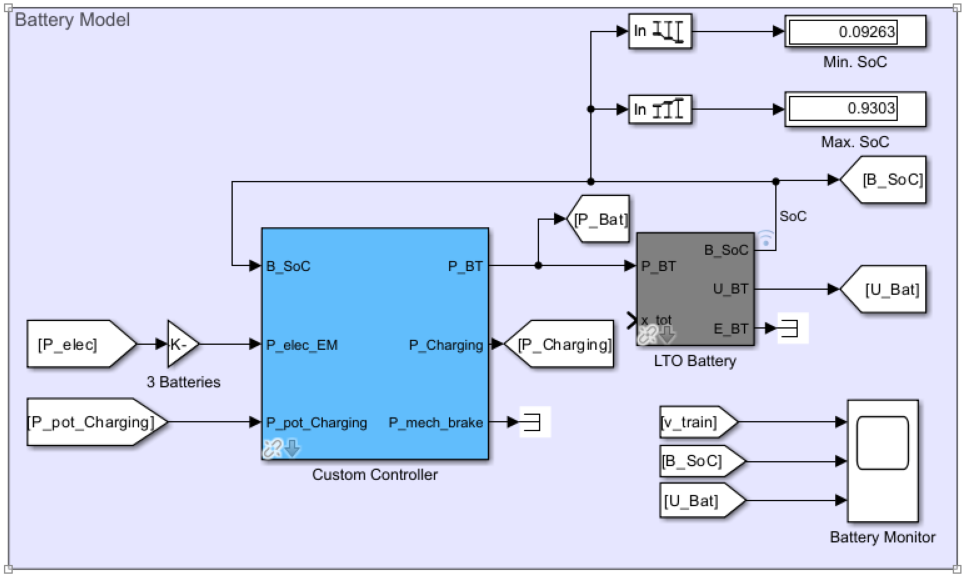
\includegraphics[width=0.7\linewidth]{EV_Project - Mauretanian Train/plots/Battery_model_ss.PNG}
    \caption{Battey model of the LTO Battery together with controller in QSS.}
    \label{fig:Battery_model}
\end{figure}

\begin{figure}[ht]
    \centering
    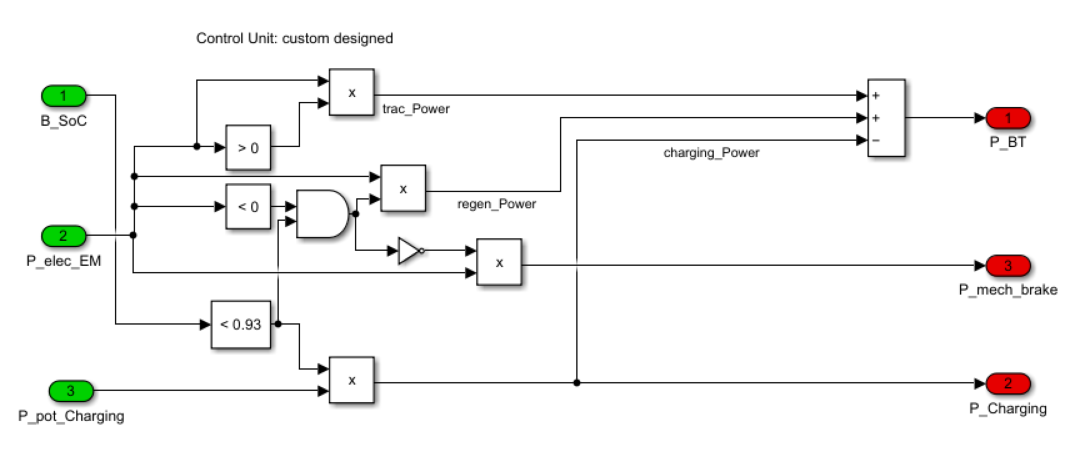
\includegraphics[width=0.7\linewidth]{EV_Project - Mauretanian Train/plots/battery_controller_ss.PNG}
    \caption{Custom battery controller, to ensure LTO battery gets not overcharged and simulation does not break.}
    \label{fig:Controller_model}
\end{figure}

\begin{figure}[ht]
    \centering
    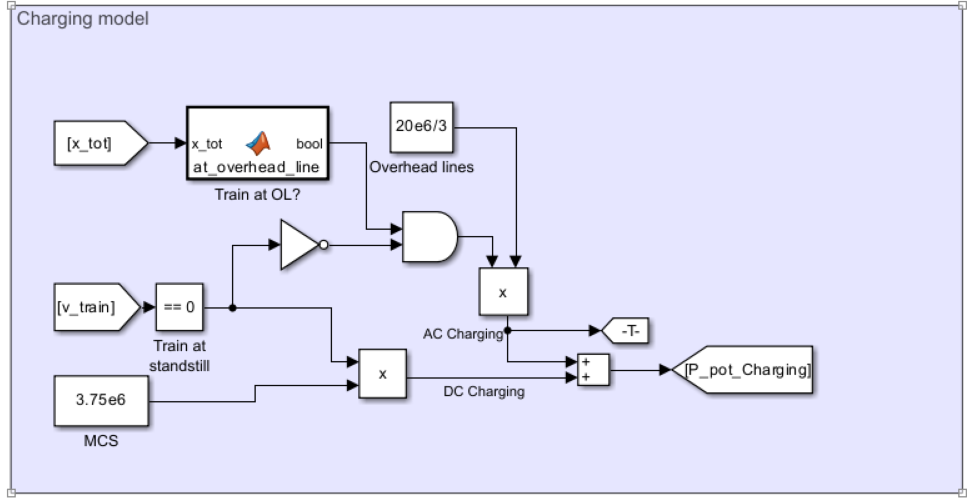
\includegraphics[width=0.7\linewidth]{EV_Project - Mauretanian Train/plots/charging_model_ss.PNG}
    \caption{Charging model of the charging island infrastructure, per battery.}
    \label{fig:Charging_model}
\end{figure}